\section{OK, now lets actually do some VHDL}\label{section:vhdl}

This section is where the majority of the instruction boxes are, as such it's very specific the to Vivado, so if you're the using a different tool at home it might not be too helpful.

\subsection{Reference Project Overview}
The reference project provided enables you to flash some LEDs at different speeds using the counter previously discussed - this demonstrates the ability to create designs with different things happening at different times and at different rates. It also contains some stubs for you to put in your own functionality; turning off and on an LED from a switch. 

\subsubsection{File Types}
A VHDL project will typically contain the following files:
\begin{enumerate}
    \item Design Source Files \texttt{*.vhd}: These contain the actual source code for the hardware you're describing. These should contain only synthesisable code.
    \item Design Test Benches \texttt{*\_tb.vhd}: These contain test benches for your design entities, usually suffixed with \texttt{\_tb} so you know it's a test bench, and will likely contain non synthesisable code.
    \item Constraints Files \texttt{*.(ucf|xcd)}: These files describe any constraints of the platform or design, such as pins used, timing requirements etc. Note that these extensions are Xilinx specific, Quartus uses \texttt{.qsd}.
    \item Scripts \texttt{*.(sh|tcl)}: These are provided to help with setting up and managing the project. \texttt{tcl} files seem to be what most tools prefer, and tools will often provide a number of utility functions to help with this. 
\end{enumerate}

\subsection{How to get started with a new design}
There are heaps of tutorials online for how to do this in all sorts of toolchains, such as this\footnote{\url{https://reference.digilentinc.com/vivado/getting_started/start}} or this\footnote{\url{https://www.intel.com/content/www/us/en/programmable/documentation/yoq1529444104707.html}} so I won't cover that here. If you're reading this and it's printed then good luck typing those in! Ask me for an electronic copy and I'll make sure you get one, alternatively google \emph{Quartus getting started} or similar.

\subsection{Open the reference project}
\subsubsection{ghdl}
This is just a command line tool, so there's no project to open. Just use vim or something to look at the files individually.

\subsubsection{Vivado}
Vivado is a pretty huge tool which produces loads of artefacts, most of which are generated by the tool so we don't need to keep them in version control. For this reason there is a \texttt{tcl} script which instructs it to setup our project again.

\instructionbox{At the terminal: \texttt{vivado create\_project}}

\subsection{Build the reference project}
\subsubsection{ghdl}
\texttt{ghdl} doesn't have an IDE or anything, so I have been using scripts to automate this build process. 

\instructionbox{\texttt{./build.sh} in the \texttt{scripts} folder}

\subsubsection{Vivado}

\subsection{Run the simulation}
\subsubsection{ghdl} 
The script you ran before already did this, if you want you can run it again.

\instructionbox{\texttt{./build.sh} in the \texttt{scripts} folder}


\instructionbox{Open it in \texttt{gtkwave}}
\\
\,
This has already been seen before in \cref{fig:counter_wave}.

\subsubsection{Vivado}

\subsection{Load onto the Device}

\subsection{Implement the architecture of the stubs}

\subsection{Device Overview}
The Zedboard is a development board based around a Xilinx Zynq-7000 device. As previously mentioned it's got 2 ARM cores on board along with a bunch of Programmable Logic (seen in \cref{fig:zynq}). It's important to be aware of this because any bitstreams and designs we produce need to include an interface to one more more of these cores. Infact for the reference project they will serve as our clock source. There are heaps of things you can use which are already built in as peripherals to the PS such as GPIO, Serial Comms and PS-PL interuppt control. The fun part about FPGAs though is learning how to do this in the Programmable Logic!

\begin{figure}[H]
    \begin{center}
        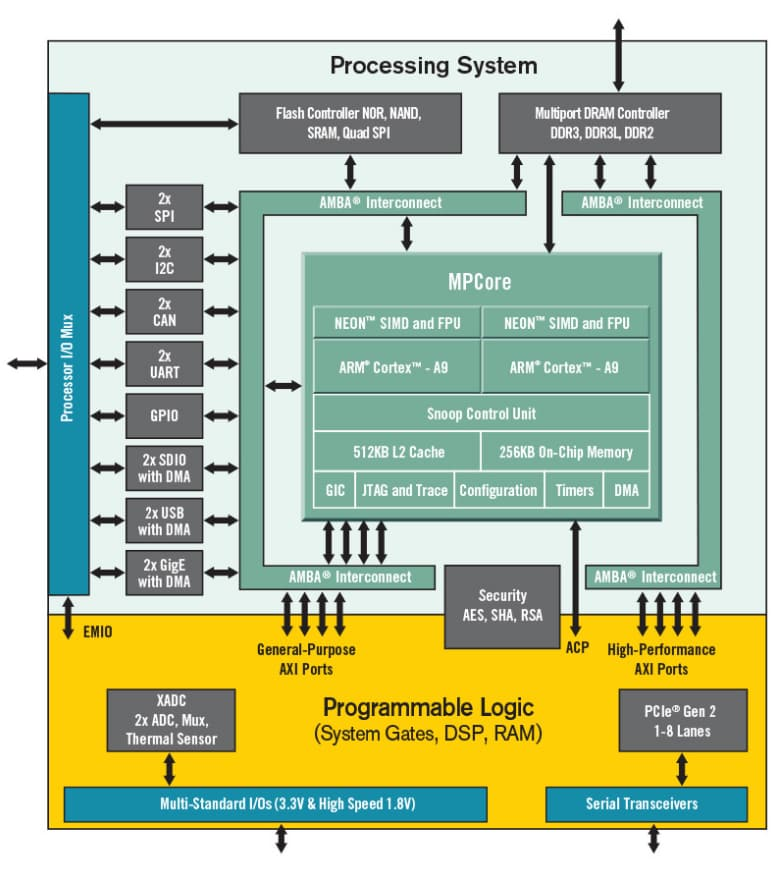
\includegraphics[width=0.7\textwidth]{./src/zynq_arch.jpg}
        \caption{The Zynq device architecture}
        \label{fig:zynq}
    \end{center}
\end{figure}

\subsubsection{How to find what connects to what}
This is an important thing to be able to do, and if you love datasheets like me you're in for a treat! First we need to identify which switches and LEDs on the physical hardware we want to use, for this I want to use slide switches 0 and 1, and LED 0. Although not marked in \cref{fig:zedoverlay} they are just above the slide switches.

\instructionbox{Find the switches and LEDs on the actual Zedboard}

\begin{figure}[H]
    \begin{center}
        \includegraphics[width=0.7\textwidth]{./src/Zedboard_Overlay.jpg}
        \caption{The Zedbaord Layout}
        \label{fig:zedoverlay}
    \end{center}
\end{figure}

The next step is to reference the schematic\footnote{Available on \url{https://www.xilinx.com}}.

\instructionbox{Find \texttt{SW0}, \texttt{SW1} and \texttt{LD0}. This can be done with a \texttt{ctrl-f} usually. These can both be found on sheet 3 of the schematic, and are shown in \cref{fig:schemled} and \cref{fig:schemsw}.}

\begin{figure}[H]
    \begin{center}
        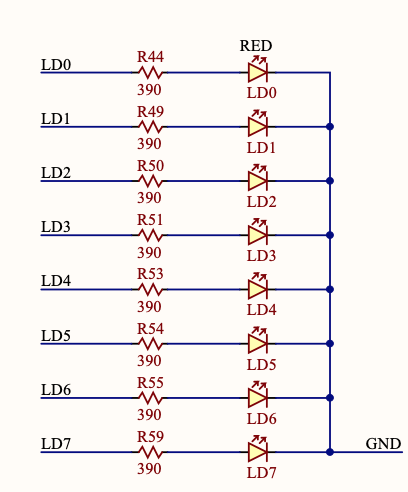
\includegraphics[width=0.4\textwidth]{./src/schem_led.png}
        \caption{The Zedboard LEDs  on the schematic}
        \label{fig:schemled}
    \end{center}
\end{figure}

\begin{figure}[H]
    \begin{center}
        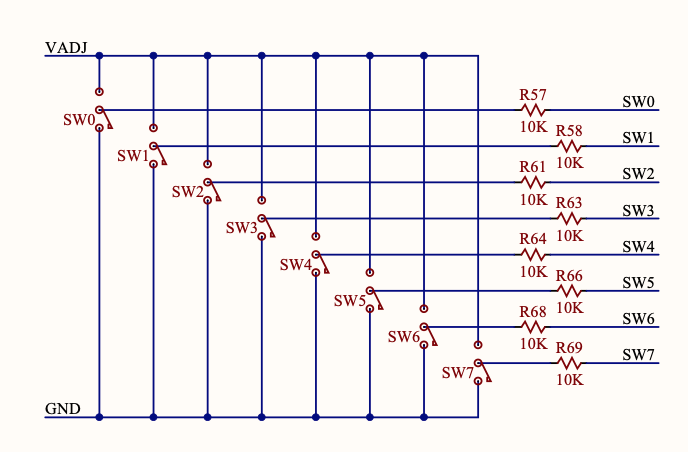
\includegraphics[width=0.5\textwidth]{./src/schem_sw.png}
        \caption{The Zedboard switches  on the schematic}
        \label{fig:schemsw}
    \end{center}
\end{figure}

On the schematic, how we have found the physical components we need to find where they connect to the FPGA BGA\footnote{Ball Grid Array - the pads attached to the FPGA IC}. This can be done by finding the other end of the \texttt{SW0} net shown on the right hand side of \cref{fig:schemsw}. It should take you to a sheet 9, and in the bottom right hand corner are the switches. Shown in \cref{fig:schembga}.


\instructionbox{Identify the BGA grid location of the connection to the FPGA}

\begin{figure}[H]
    \begin{center}
        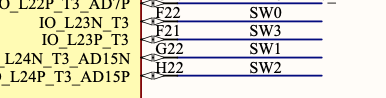
\includegraphics[width=0.5\textwidth]{./src/schem_bga.png}
        \caption{The Zedboard switches connect to the FPGA at BGA location F22 and G22}
        \label{fig:schembga}
    \end{center}
\end{figure}

%------------------------------------------------------------------------------------------------------------------------------------------------------
\section{Further Activities}\label{section:fa}
If this has been fun, and you want to learn more here are some useful resources I have had successes with:

\begin{itemize}
    \item Effective Coding with VHDL\footnote{\url{https://www.amazon.co.uk/Effective-Coding-VHDL-Principles-Practice/dp/0262034220}} 
    \item Awesome VHDL\footnote{\url{https://github.com/VHDL/awesome-vhdl}}
    \item Digital Fundamentals\footnote{\url{https://www.amazon.co.uk/Digital-Fundamentals-Thomas-L-Floyd/dp/0132737965}}
    \item Doulos Guide\footnote{\url{https://www.ics.uci.edu/~jmoorkan/vhdlref/vhdl_golden_reference_guide.pdf}}
\end{itemize}
